\documentclass[12pt, a4paper]{article}\usepackage[]{graphicx}\usepackage[]{color}
% maxwidth is the original width if it is less than linewidth
% otherwise use linewidth (to make sure the graphics do not exceed the margin)
\makeatletter
\def\maxwidth{ %
  \ifdim\Gin@nat@width>\linewidth
    \linewidth
  \else
    \Gin@nat@width
  \fi
}
\makeatother

\definecolor{fgcolor}{rgb}{0.345, 0.345, 0.345}
\makeatletter
\@ifundefined{AddToHook}{}{\AddToHook{package/xcolor/after}{\definecolor{fgcolor}{rgb}{0.345, 0.345, 0.345}}}
\makeatother
\newcommand{\hlnum}[1]{\textcolor[rgb]{0.686,0.059,0.569}{#1}}%
\newcommand{\hlstr}[1]{\textcolor[rgb]{0.192,0.494,0.8}{#1}}%
\newcommand{\hlcom}[1]{\textcolor[rgb]{0.678,0.584,0.686}{\textit{#1}}}%
\newcommand{\hlopt}[1]{\textcolor[rgb]{0,0,0}{#1}}%
\newcommand{\hlstd}[1]{\textcolor[rgb]{0.345,0.345,0.345}{#1}}%
\newcommand{\hlkwa}[1]{\textcolor[rgb]{0.161,0.373,0.58}{\textbf{#1}}}%
\newcommand{\hlkwb}[1]{\textcolor[rgb]{0.69,0.353,0.396}{#1}}%
\newcommand{\hlkwc}[1]{\textcolor[rgb]{0.333,0.667,0.333}{#1}}%
\newcommand{\hlkwd}[1]{\textcolor[rgb]{0.737,0.353,0.396}{\textbf{#1}}}%
\let\hlipl\hlkwb

\usepackage{framed}
\makeatletter
\newenvironment{kframe}{%
 \def\at@end@of@kframe{}%
 \ifinner\ifhmode%
  \def\at@end@of@kframe{\end{minipage}}%
  \begin{minipage}{\columnwidth}%
 \fi\fi%
 \def\FrameCommand##1{\hskip\@totalleftmargin \hskip-\fboxsep
 \colorbox{shadecolor}{##1}\hskip-\fboxsep
     % There is no \\@totalrightmargin, so:
     \hskip-\linewidth \hskip-\@totalleftmargin \hskip\columnwidth}%
 \MakeFramed {\advance\hsize-\width
   \@totalleftmargin\z@ \linewidth\hsize
   \@setminipage}}%
 {\par\unskip\endMakeFramed%
 \at@end@of@kframe}
\makeatother

\definecolor{shadecolor}{rgb}{.97, .97, .97}
\definecolor{messagecolor}{rgb}{0, 0, 0}
\definecolor{warningcolor}{rgb}{1, 0, 1}
\definecolor{errorcolor}{rgb}{1, 0, 0}
\makeatletter
\@ifundefined{AddToHook}{}{\AddToHook{package/xcolor/after}{
\definecolor{shadecolor}{rgb}{.97, .97, .97}
\definecolor{messagecolor}{rgb}{0, 0, 0}
\definecolor{warningcolor}{rgb}{1, 0, 1}
\definecolor{errorcolor}{rgb}{1, 0, 0}
}}
\makeatother
\newenvironment{knitrout}{}{} % an empty environment to be redefined in TeX

\usepackage{alltt}

%%%%%%%%%%%%%%%%%%%%%%%%%%%%%%%%%%%%%%%%%%%%%%%%%%%%%%%%%%%%%%%%%%%%%%%%%%%%%%%%%%%%%%%%%%%%%%%%
  % dodatkowe pakiety LaTeX'a
\usepackage[OT4]{polski}
\usepackage[utf8]{inputenc}
\usepackage[top=2.5cm, bottom=2.5cm, left=2cm, right=2cm]{geometry}
\usepackage{graphicx}
\usepackage{float}
\usepackage[colorlinks=true, linkcolor=blue]{hyperref}
\usepackage{mathtools}


%%%%%%%%%%%%%%%%%%%%%%%%%%%%%%%%%%%%%%%%%%%%%%%%%%%%%%%%%%%%%%%%%%%%%%%%%%%%%%%%%%%%%%%%%%%%%%%%
% ustawienia globalne


\IfFileExists{upquote.sty}{\usepackage{upquote}}{}
\begin{document}

%%%%%%%%%%%%%%%%%%%%%%%%%%%%%%%%%%%%%%%%%%%%%%%%%%%%%%%%%%%%%%%%
  % strona tytulowa
\title{Sprawozdanie 5}
\author{Maciej Łosiewicz \\ album 256319}
\maketitle


\section{Zadanie  1}

W tym zadaniu zweryfikujemy hipotezę istotności (a właściwie nieistotności) zmiennej $meal.cal$
w przyjętym modelu.

\begin{knitrout}
\definecolor{shadecolor}{rgb}{0.969, 0.969, 0.969}\color{fgcolor}\begin{kframe}
\begin{alltt}
\hlstd{df} \hlkwb{<-} \hlstd{lung}
\hlstd{df[}\hlstr{"status"}\hlstd{][df[}\hlstr{"status"}\hlstd{]} \hlopt{==} \hlnum{1}\hlstd{]} \hlkwb{<-} \hlnum{0}
\hlstd{df[}\hlstr{"status"}\hlstd{][df[}\hlstr{"status"}\hlstd{]} \hlopt{==} \hlnum{2}\hlstd{]} \hlkwb{<-} \hlnum{1}
\hlstd{df} \hlkwb{<-} \hlkwd{na.omit}\hlstd{(df)}
\hlkwd{attach}\hlstd{(df)}


\hlstd{fit} \hlkwb{<-} \hlkwd{coxph}\hlstd{(}\hlkwd{Surv}\hlstd{(time, status)} \hlopt{~} \hlstd{age} \hlopt{+} \hlstd{sex} \hlopt{+} \hlstd{ph.ecog} \hlopt{+}
               \hlstd{ph.karno} \hlopt{+} \hlstd{pat.karno} \hlopt{+} \hlstd{meal.cal} \hlopt{+} \hlstd{wt.loss,} \hlkwc{data} \hlstd{= df)}

\hlkwd{summary}\hlstd{(fit)}
\end{alltt}
\begin{verbatim}
## Call:
## coxph(formula = Surv(time, status) ~ age + sex + ph.ecog + ph.karno + 
##     pat.karno + meal.cal + wt.loss, data = df)
## 
##   n= 167, number of events= 120 
## 
##                 coef  exp(coef)   se(coef)      z Pr(>|z|)   
## age        1.080e-02  1.011e+00  1.160e-02  0.931  0.35168   
## sex       -5.536e-01  5.749e-01  2.016e-01 -2.746  0.00603 **
## ph.ecog    7.395e-01  2.095e+00  2.250e-01  3.287  0.00101 **
## ph.karno   2.244e-02  1.023e+00  1.123e-02  1.998  0.04575 * 
## pat.karno -1.207e-02  9.880e-01  8.116e-03 -1.488  0.13685   
## meal.cal   2.835e-05  1.000e+00  2.594e-04  0.109  0.91298   
## wt.loss   -1.420e-02  9.859e-01  7.766e-03 -1.828  0.06748 . 
## ---
## Signif. codes:  0 '***' 0.001 '**' 0.01 '*' 0.05 '.' 0.1 ' ' 1
## 
##           exp(coef) exp(-coef) lower .95 upper .95
## age          1.0109     0.9893    0.9881    1.0341
## sex          0.5749     1.7395    0.3872    0.8534
## ph.ecog      2.0950     0.4773    1.3479    3.2560
## ph.karno     1.0227     0.9778    1.0004    1.0455
## pat.karno    0.9880     1.0121    0.9724    1.0038
## meal.cal     1.0000     1.0000    0.9995    1.0005
## wt.loss      0.9859     1.0143    0.9710    1.0010
## 
## Concordance= 0.653  (se = 0.029 )
## Likelihood ratio test= 28.16  on 7 df,   p=2e-04
## Wald test            = 27.5  on 7 df,   p=3e-04
## Score (logrank) test = 28.31  on 7 df,   p=2e-04
\end{verbatim}
\end{kframe}
\end{knitrout}

Wartość $p.value$ dla zmiennej $meal.cal$ wynosi 0.91, co mocno wskazuje na $H_0$.
\section{Zadanie 2}

Tak samo jak poprzednie zadanie, tylko w tym wypadku będziemy badać zmienną $pat.karno$

\begin{knitrout}
\definecolor{shadecolor}{rgb}{0.969, 0.969, 0.969}\color{fgcolor}\begin{kframe}
\begin{alltt}
\hlkwd{summary}\hlstd{(fit)}
\end{alltt}
\begin{verbatim}
## Call:
## coxph(formula = Surv(time, status) ~ age + sex + ph.ecog + ph.karno + 
##     pat.karno + meal.cal + wt.loss, data = df)
## 
##   n= 167, number of events= 120 
## 
##                 coef  exp(coef)   se(coef)      z Pr(>|z|)   
## age        1.080e-02  1.011e+00  1.160e-02  0.931  0.35168   
## sex       -5.536e-01  5.749e-01  2.016e-01 -2.746  0.00603 **
## ph.ecog    7.395e-01  2.095e+00  2.250e-01  3.287  0.00101 **
## ph.karno   2.244e-02  1.023e+00  1.123e-02  1.998  0.04575 * 
## pat.karno -1.207e-02  9.880e-01  8.116e-03 -1.488  0.13685   
## meal.cal   2.835e-05  1.000e+00  2.594e-04  0.109  0.91298   
## wt.loss   -1.420e-02  9.859e-01  7.766e-03 -1.828  0.06748 . 
## ---
## Signif. codes:  0 '***' 0.001 '**' 0.01 '*' 0.05 '.' 0.1 ' ' 1
## 
##           exp(coef) exp(-coef) lower .95 upper .95
## age          1.0109     0.9893    0.9881    1.0341
## sex          0.5749     1.7395    0.3872    0.8534
## ph.ecog      2.0950     0.4773    1.3479    3.2560
## ph.karno     1.0227     0.9778    1.0004    1.0455
## pat.karno    0.9880     1.0121    0.9724    1.0038
## meal.cal     1.0000     1.0000    0.9995    1.0005
## wt.loss      0.9859     1.0143    0.9710    1.0010
## 
## Concordance= 0.653  (se = 0.029 )
## Likelihood ratio test= 28.16  on 7 df,   p=2e-04
## Wald test            = 27.5  on 7 df,   p=3e-04
## Score (logrank) test = 28.31  on 7 df,   p=2e-04
\end{verbatim}
\end{kframe}
\end{knitrout}

Wartość $p.value$ dla zmiennej $pat.karno$ wynosi 0.13, co mocno wskazuje na $H_0$.

\section{Zadanie 3}

Korzystając z funkcji step dokonamy wyboru zmiennych do modelu Coxa korzystając z (a) kryterium
informacyjnego Akaike’a (AIC), oraz (b) kryterium BIC.

AIC: 

\begin{knitrout}
\definecolor{shadecolor}{rgb}{0.969, 0.969, 0.969}\color{fgcolor}\begin{kframe}
\begin{alltt}
\hlstd{AIC} \hlkwb{<-} \hlkwd{step}\hlstd{(fit,} \hlkwc{k} \hlstd{=} \hlnum{2}\hlstd{,} \hlkwc{scope} \hlstd{=} \hlkwd{list}\hlstd{(}\hlkwc{upper} \hlstd{=} \hlopt{~}\hlstd{.,} \hlkwc{lower} \hlstd{=} \hlopt{~}\hlnum{1}\hlstd{))}
\end{alltt}
\begin{verbatim}
## Start:  AIC=1002.07
## Surv(time, status) ~ age + sex + ph.ecog + ph.karno + pat.karno + 
##     meal.cal + wt.loss
## 
##             Df    AIC
## - meal.cal   1 1000.1
## - age        1 1001.0
## <none>         1002.1
## - pat.karno  1 1002.3
## - wt.loss    1 1003.6
## - ph.karno   1 1004.3
## - sex        1 1008.0
## - ph.ecog    1 1011.1
## 
## Step:  AIC=1000.08
## Surv(time, status) ~ age + sex + ph.ecog + ph.karno + pat.karno + 
##     wt.loss
## 
##             Df     AIC
## - age        1  998.95
## <none>         1000.08
## - pat.karno  1 1000.29
## - wt.loss    1 1001.60
## + meal.cal   1 1002.07
## - ph.karno   1 1002.28
## - sex        1 1006.29
## - ph.ecog    1 1009.09
## 
## Step:  AIC=998.95
## Surv(time, status) ~ sex + ph.ecog + ph.karno + pat.karno + wt.loss
## 
##             Df     AIC
## <none>          998.95
## - pat.karno  1  999.34
## + age        1 1000.08
## - ph.karno   1 1000.53
## - wt.loss    1 1000.74
## + meal.cal   1 1000.95
## - sex        1 1005.25
## - ph.ecog    1 1007.83
\end{verbatim}
\end{kframe}
\end{knitrout}

BIC: 

\begin{knitrout}
\definecolor{shadecolor}{rgb}{0.969, 0.969, 0.969}\color{fgcolor}\begin{kframe}
\begin{alltt}
\hlstd{BIC} \hlkwb{<-} \hlkwd{step}\hlstd{(fit,} \hlkwc{k} \hlstd{=} \hlkwd{log}\hlstd{(}\hlkwd{length}\hlstd{(df[,}\hlnum{1}\hlstd{])),} \hlkwc{scope} \hlstd{=} \hlkwd{list}\hlstd{(}\hlkwc{upper} \hlstd{=} \hlopt{~}\hlstd{.,} \hlkwc{lower} \hlstd{=} \hlopt{~}\hlnum{1}\hlstd{))}
\end{alltt}
\begin{verbatim}
## Start:  AIC=1023.89
## Surv(time, status) ~ age + sex + ph.ecog + ph.karno + pat.karno + 
##     meal.cal + wt.loss
## 
##             Df    AIC
## - meal.cal   1 1018.8
## - age        1 1019.7
## - pat.karno  1 1021.0
## - wt.loss    1 1022.3
## - ph.karno   1 1023.0
## <none>         1023.9
## - sex        1 1026.7
## - ph.ecog    1 1029.8
## 
## Step:  AIC=1018.79
## Surv(time, status) ~ age + sex + ph.ecog + ph.karno + pat.karno + 
##     wt.loss
## 
##             Df    AIC
## - age        1 1014.5
## - pat.karno  1 1015.9
## - wt.loss    1 1017.2
## - ph.karno   1 1017.9
## <none>         1018.8
## - sex        1 1021.9
## + meal.cal   1 1023.9
## - ph.ecog    1 1024.7
## 
## Step:  AIC=1014.54
## Surv(time, status) ~ sex + ph.ecog + ph.karno + pat.karno + wt.loss
## 
##             Df    AIC
## - pat.karno  1 1011.8
## - ph.karno   1 1013.0
## - wt.loss    1 1013.2
## <none>         1014.5
## - sex        1 1017.7
## + age        1 1018.8
## + meal.cal   1 1019.7
## - ph.ecog    1 1020.3
## 
## Step:  AIC=1011.81
## Surv(time, status) ~ sex + ph.ecog + ph.karno + wt.loss
## 
##             Df    AIC
## - wt.loss    1 1009.4
## - ph.karno   1 1009.5
## <none>         1011.8
## + pat.karno  1 1014.5
## - sex        1 1015.4
## + age        1 1015.9
## + meal.cal   1 1016.8
## - ph.ecog    1 1022.0
## 
## Step:  AIC=1009.43
## Surv(time, status) ~ sex + ph.ecog + ph.karno
## 
##             Df    AIC
## - ph.karno   1 1007.0
## <none>         1009.4
## + wt.loss    1 1011.8
## - sex        1 1012.0
## + pat.karno  1 1013.2
## + age        1 1013.2
## + meal.cal   1 1014.4
## - ph.ecog    1 1017.2
## 
## Step:  AIC=1006.99
## Surv(time, status) ~ sex + ph.ecog
## 
##             Df    AIC
## <none>         1007.0
## - sex        1 1008.9
## + ph.karno   1 1009.4
## + wt.loss    1 1009.5
## + pat.karno  1 1011.2
## + age        1 1011.6
## + meal.cal   1 1012.0
## - ph.ecog    1 1015.1
\end{verbatim}
\end{kframe}
\end{knitrout}

\section{Zadanie 4}

Naszkicujemy wykres funkcji hazardu i funkcji przeżycia odpowiadające jednostce o wybranych charakterystykach na podstawie modelu wybranego w poprzednim punkcie przy kryterium AIC.


Funkcja hazardu:

\begin{knitrout}
\definecolor{shadecolor}{rgb}{0.969, 0.969, 0.969}\color{fgcolor}\begin{kframe}
\begin{alltt}
\hlkwd{ggsurvplot}\hlstd{(}\hlkwd{survfit}\hlstd{(AIC),} \hlkwc{data} \hlstd{= df)}
\end{alltt}
\end{kframe}

{\centering 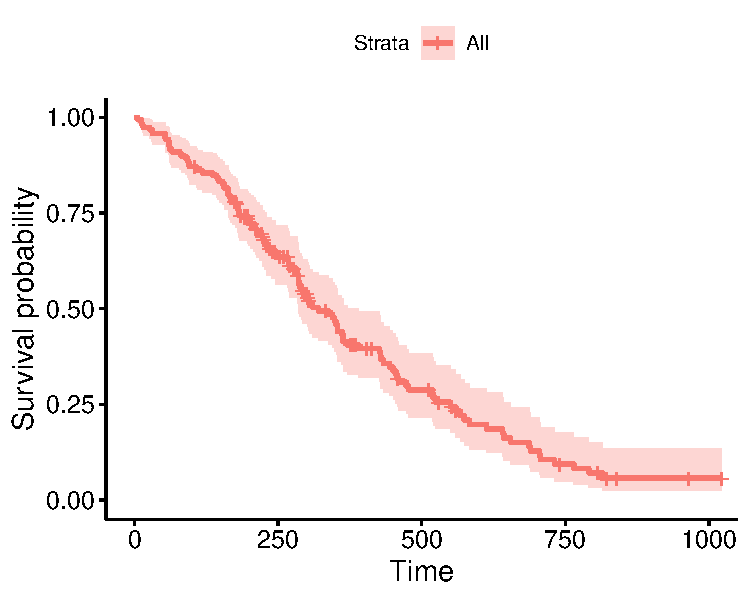
\includegraphics[width=\maxwidth]{figure/unnamed-chunk-5-1} 

}


\end{knitrout}


Funkcja przeżycia:

\begin{knitrout}
\definecolor{shadecolor}{rgb}{0.969, 0.969, 0.969}\color{fgcolor}\begin{kframe}
\begin{alltt}
\hlkwd{plot}\hlstd{(}\hlkwd{basehaz}\hlstd{(AIC,} \hlkwc{centered} \hlstd{= T))}
\end{alltt}
\end{kframe}

{\centering 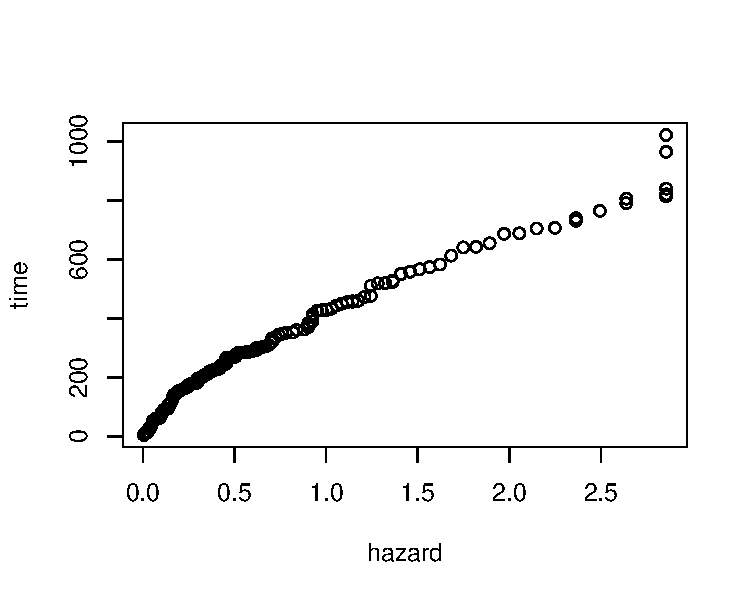
\includegraphics[width=\maxwidth]{figure/unnamed-chunk-6-1} 

}


\end{knitrout}

\section{Zadanie 5}

Na koniec zweryfikujemy hipotezę o proporcjonalności hazardów. Zastanowimy się nad problemem “momentu”,
w którym tą hipotezę powinniśmy weryfikować.
\begin{knitrout}
\definecolor{shadecolor}{rgb}{0.969, 0.969, 0.969}\color{fgcolor}\begin{kframe}
\begin{alltt}
\hlkwd{cox.zph}\hlstd{(AIC)}
\end{alltt}
\begin{verbatim}
##            chisq df     p
## sex       1.3921  1 0.238
## ph.ecog   3.3422  1 0.068
## ph.karno  5.9111  1 0.015
## pat.karno 3.1717  1 0.075
## wt.loss   0.0933  1 0.760
## GLOBAL    8.0599  5 0.153
\end{verbatim}
\end{kframe}
\end{knitrout}



\section{Zadanie 6}

W tym zadaniu dopasujemy model proporcjonalności szans.

\begin{knitrout}
\definecolor{shadecolor}{rgb}{0.969, 0.969, 0.969}\color{fgcolor}\begin{kframe}
\begin{alltt}
\hlstd{modelprop} \hlkwb{<-} \hlkwd{prop.odds}\hlstd{(}\hlkwd{Event}\hlstd{(time, status)} \hlopt{~} \hlstd{age} \hlopt{+} \hlstd{sex} \hlopt{+} \hlstd{ph.ecog} \hlopt{+}
                         \hlstd{ph.karno} \hlopt{+} \hlstd{pat.karno} \hlopt{+} \hlstd{meal.cal} \hlopt{+} \hlstd{wt.loss,} \hlkwc{data} \hlstd{= df)}
\hlstd{modelprop}\hlopt{$}\hlstd{gamma}
\end{alltt}
\begin{verbatim}
##                estimate
## age        0.0030308659
## sex       -1.0150375581
## ph.ecog    0.8947795967
## ph.karno   0.0130517401
## pat.karno -0.0153372382
## meal.cal  -0.0004122679
## wt.loss   -0.0135972811
\end{verbatim}
\end{kframe}
\end{knitrout}


\section{Zadanie 7}

Teraz powtórzymy zadanie 6, ale bez zmiennych $age$ oraz $meal.cal$

\begin{knitrout}
\definecolor{shadecolor}{rgb}{0.969, 0.969, 0.969}\color{fgcolor}\begin{kframe}
\begin{alltt}
\hlstd{modelprop1} \hlkwb{<-} \hlkwd{prop.odds}\hlstd{(}\hlkwd{Event}\hlstd{(time, status)} \hlopt{~} \hlstd{sex} \hlopt{+} \hlstd{ph.ecog} \hlopt{+}
                         \hlstd{ph.karno} \hlopt{+} \hlstd{pat.karno} \hlopt{+} \hlstd{wt.loss,} \hlkwc{data} \hlstd{= df)}
\hlstd{modelprop1}\hlopt{$}\hlstd{gamma}
\end{alltt}
\begin{verbatim}
##              estimate
## sex       -0.96878081
## ph.ecog    0.91767146
## ph.karno   0.01350458
## pat.karno -0.01683724
## wt.loss   -0.01318218
\end{verbatim}
\end{kframe}
\end{knitrout}

\section{Zadanie 8 oraz 9}
Teraz, zweryfikujemy hipotęzę o istotności zmiennej $meal.cal$ w przyjętym modelu.
\begin{knitrout}
\definecolor{shadecolor}{rgb}{0.969, 0.969, 0.969}\color{fgcolor}\begin{kframe}
\begin{alltt}
\hlstd{modelprop}
\end{alltt}
\begin{verbatim}
## Proportional Odds model 
## 
## Test for baseline 
## Test for nonparametric terms 
## 
## Test for non-significant effects 
##          Supremum-test of significance p-value H_0: B(t)=0
## Baseline                         0.327               0.914
## 
## Test for time invariant effects 
##                Kolmogorov-Smirnov test p-value H_0:constant effect
## Baseline                          19.7                       0.786
## 
## Covariate effects 
##               Coef.       SE Robust SE D2log(L)^-1      z   P-val lower2.5%
## age        0.003030 0.017400  0.017200    0.017300  0.177 0.86000  -0.03110
## sex       -1.020000 0.328000  0.349000    0.322000 -2.910 0.00367  -1.66000
## ph.ecog    0.895000 0.396000  0.433000    0.373000  2.070 0.03860   0.11900
## ph.karno   0.013100 0.023100  0.028400    0.021900  0.459 0.64600  -0.03220
## pat.karno -0.015300 0.012500  0.012500    0.011700 -1.230 0.22000  -0.03980
## meal.cal  -0.000412 0.000397  0.000388    0.000376 -1.060 0.28800  -0.00119
## wt.loss   -0.013600 0.011300  0.010800    0.010700 -1.260 0.20800  -0.03570
##           upper97.5%
## age         0.037100
## sex        -0.377000
## ph.ecog     1.670000
## ph.karno    0.058400
## pat.karno   0.009200
## meal.cal    0.000366
## wt.loss     0.008550
## Test of Goodness-of-fit 
##           sup|  hat U(t) | p-value H_0 
## age                  80.90        0.046
## sex                   2.14        0.688
## ph.ecog               3.34        0.700
## ph.karno             78.20        0.348
## pat.karno            79.40        0.554
## meal.cal           2820.00        0.224
## wt.loss              79.90        0.372
\end{verbatim}
\end{kframe}
\end{knitrout}
Wartość $p.value$ dla zmiennej $meal.cal$ wynosi 0.288, co mocno wskazuje na $H_0$.
Wartość $p.value$ dla zmiennej $pat.karno$ wynosi 0.646, co także wskazuje na $H_0$


\end{document}
